\newpage
\section{Auswertung}

    \subsection{Untersuchung von Quarzkügelchen}




    \subsection{Untersuchung des Vesikeltransports in Zwiebeln}
        \FloatBarrier
        Zur Charakterisierung der Vesikel werden zunächst die Größen der vier in Abbildung \ref{fig:vesikel_size} rot hervorgehobenen Vesikel bestimmt. Dazu wird der Durchmesser der Vesikel über eine 
        Bildbearbeitungssoftware in der Einheit pixel bestimmt und anschließend über die in Abschnitt REF berechnete Größe eines Pixels im Realraum zu den in Tabelle \ref{tab:d_vesikel} aufgelisteten Werten 
        umgerechnet. Im Mittel ergibt sich so ein Vesikeldurchmesser d$_\text{Vesikel}$ von \SI{0.705}{\micro\metre}.
        %
        \begin{table}[h]
            \centering
            \caption{Die Durchmesser der 4 vermessenen Vesikel in der Einheit von Pixeln und im Realraum}
            \label{tab:d_vesikel}
            \begin{tabular}{c c}
            \toprule
            {d$_\text{Vesikel}$ [Pixel]} & {d$_\text{Vesikel}$ [$\mu$m]}  \\
            \midrule
            21	 &  0.666  \\
            19	 &  0.602  \\
            21	 &  0.666  \\
            28	 &  0.887  \\
            \bottomrule
            \end{tabular}
        \end{table}
        %
        \begin{figure}[h]
        \centering
        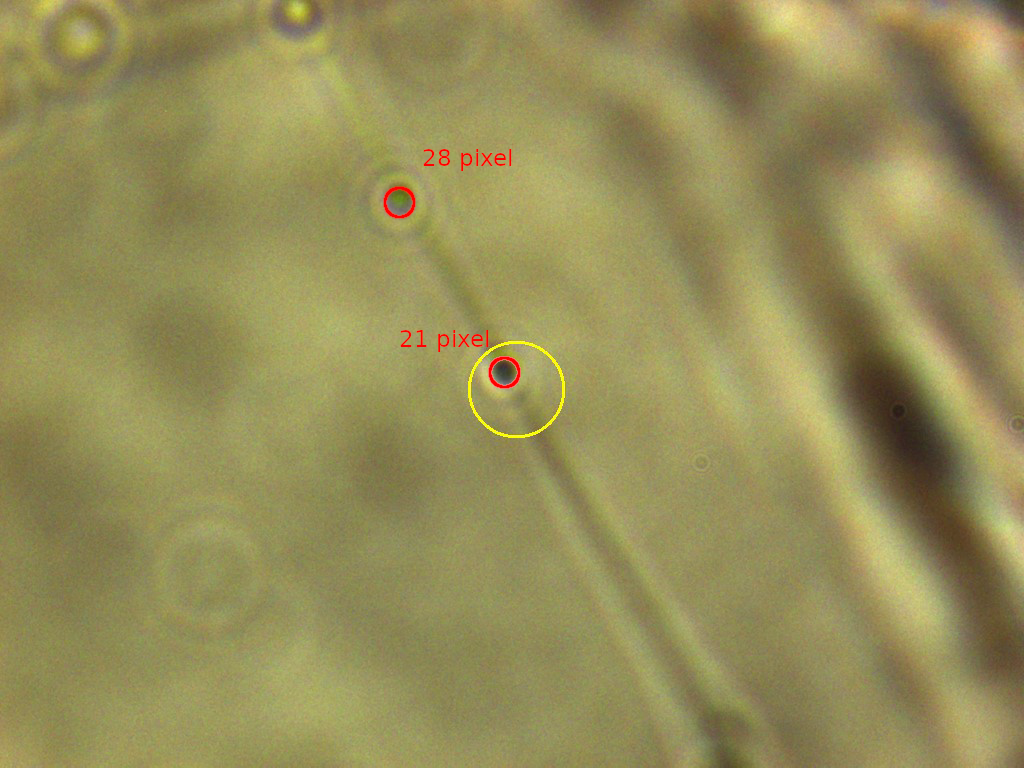
\includegraphics[width = 0.4\textwidth]{pictures/vesikel_size_1.png}
        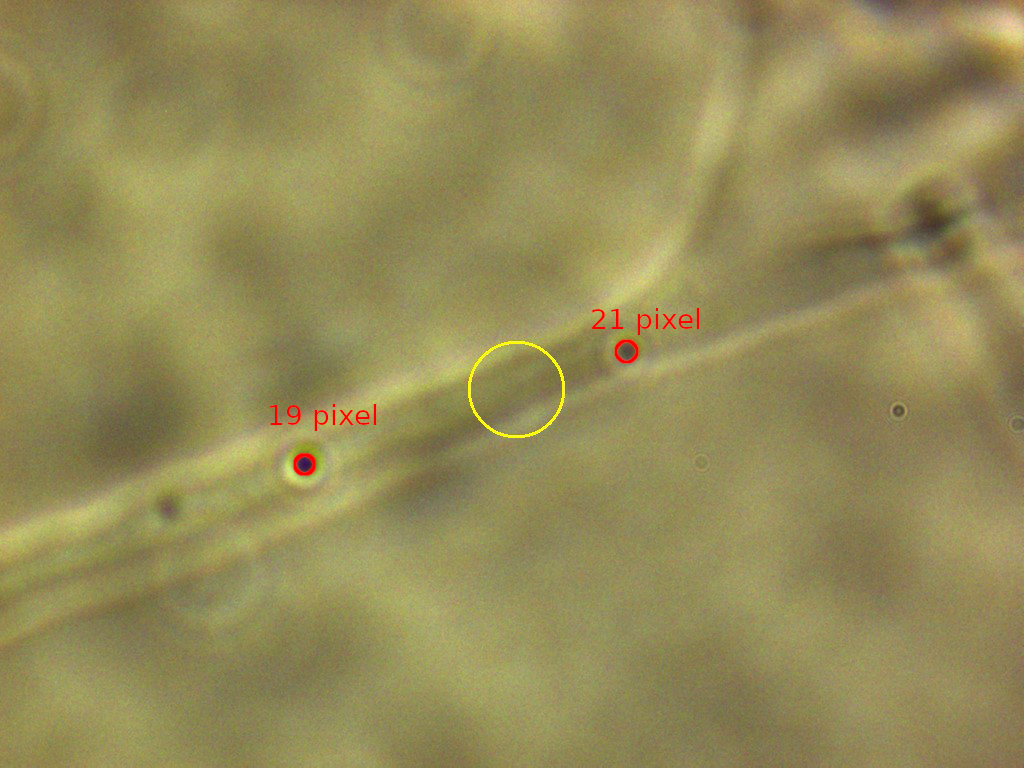
\includegraphics[width = 0.4\textwidth]{pictures/vesikel_size_2.png}
        \caption{Abbildung der vier vermessenden Vesikel, die rot hervorgehoben und deren Größe in Pixeln angegeben sind.}
        \label{fig:vesikel_size}
        \end{figure}

        \FloatBarrier
        %
        \newpage
        Zur Bestimmung der Geschwindigkeit des Vesikeltransports ist die Intensität der Photodiode gegen die Zeit beim Durchlauf eines Vesikels durch die optische Falle in Abbildung 
        \ref{fig:vesikel_size} aufgetragen. Daraus geht eine Durchquerungszeit $\Delta$t von \SI{1}{\second} hervor, die auf eine Vesikelgeschwindigkeit von 
        %
        \begin{equation*}
            v_{\text{Vesikel}} = \frac{2\text{d}_\text{Vesikel}}{\Delta\text{t}} = \SI{1.410}{\micro\metre\per\second}
        \end{equation*}
        %
        schließen lässt.
        %
        \FloatBarrier
        %
        \begin{figure}[h]
        \centering
        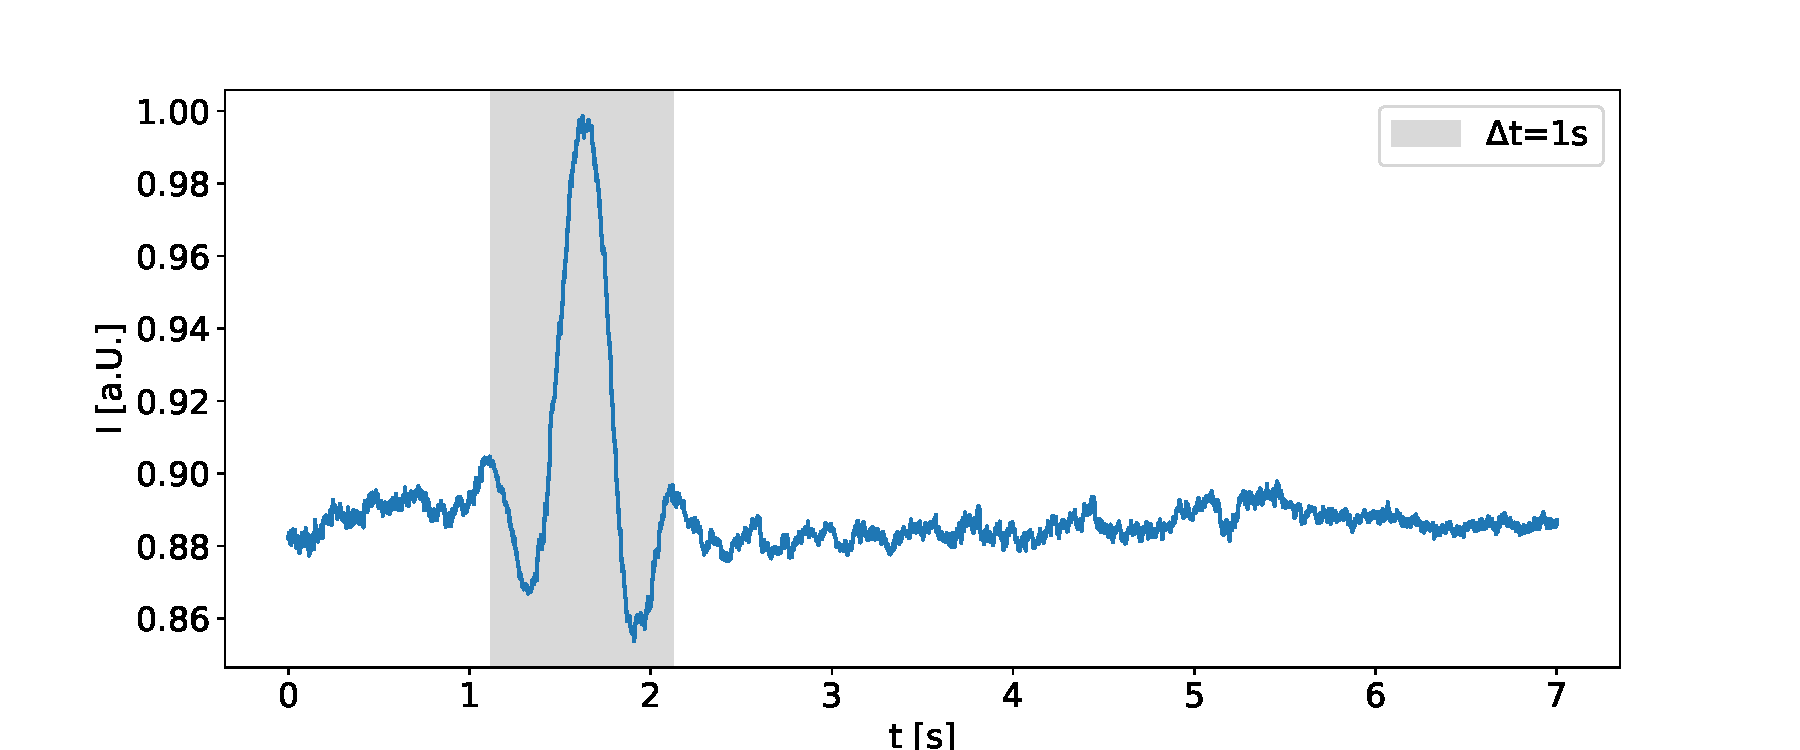
\includegraphics[width = 0.8\textwidth]{v_vesikel.pdf}
        \caption{Auf die Dauer einer Sekunde bestimmte Intensitätsänderung aufgrund des Durchlaufens eines Vesikels durch die optische Falle.}
        \label{fig:v_vesikel}
        \end{figure}
        %
        \FloatBarrier
        %
        \newpage
        Aus den restlichen Videoaufnahmen lassen sich weitere Schlüssel über das typische Verhalten des Vesikeltransports ziehen. So laufen entlang einer Actin-"Straße" alle Vesikel entlang einer Richtung
        und überholen sich nicht. Wenn ein Vesikel mit Hilfe der optischen Pinzette gegriffen wird, kann es, wie in Abbildung \ref{fig:vesikel_abstand} zu sehen, über \SI{16}{\micro\metre} weit von der 
        Actin-"Straße" entfernt werden, ohne dass sich die Bindung der Myosin-Motoren zwischen der Straße und dem Vesikel lösen. Bei Deaktivieren der optischen Pinzette springt das Vesikel zunächst zurück 
        an seine alte Position und läuft dann weiter in die ursprüngliche Richtung. 
        %
        \FloatBarrier
        %
        \begin{figure}[h]
        \centering
        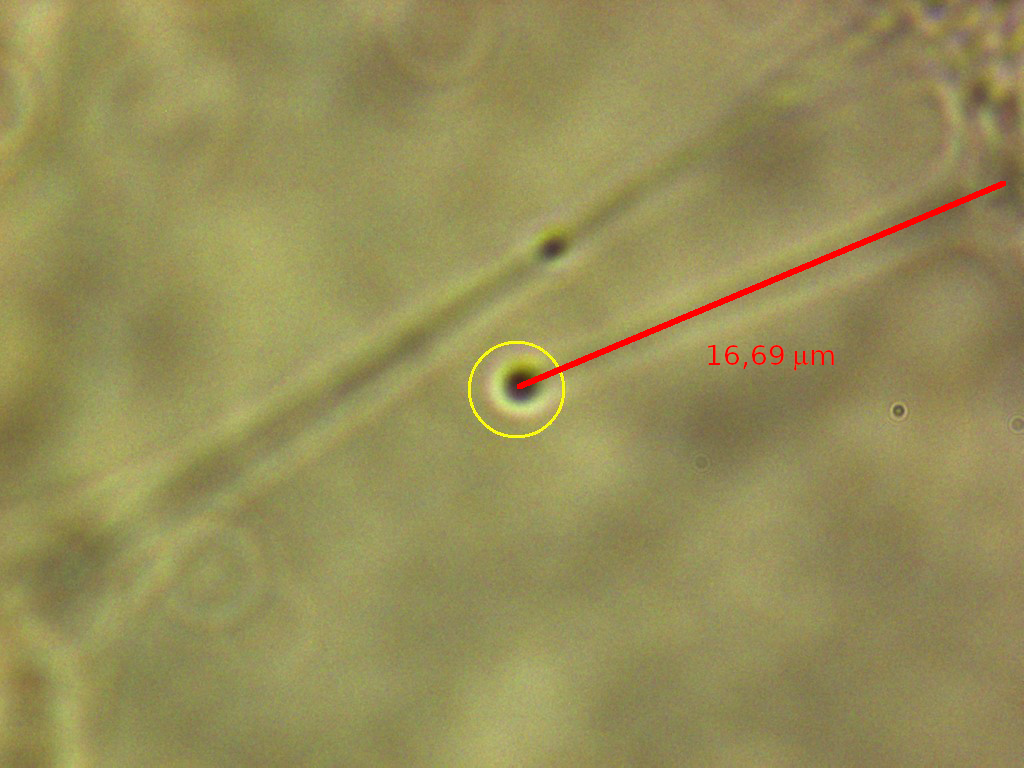
\includegraphics[width = 0.4\textwidth]{pictures/vesikel_abstand.png}
        \caption{Ein Vesikel, das über \SI{16}{\micro\metre} von seiner Ausgangsposition auf der Actin-Straße entfernt wurde.}
        \label{fig:vesikel_abstand}
        \end{figure}
        %
        \FloatBarrier 
        %
        Da die Verbindung der Myosin-Motoren nicht gebrochen werden kann, war es auch nicht möglich Vesikel von einer Straße durch Bereiche ohne Straße auf eine andere zu transferieren. Dies ist in Abbildung
        \ref{fig:vesikel_overlap} zu sehen. Ein Vesikel wird von der Straße am rechten Ende der roten Linie abgefangen und direkt über der blauen Straße platziert. Beim Deaktivieren der optischen Falle geht das 
        Vesikel auf seine Ausgangsposition auf der ehemaligen Straße zurück. 
        %
        \FloatBarrier
        %
        \begin{figure}[h]
        \centering
        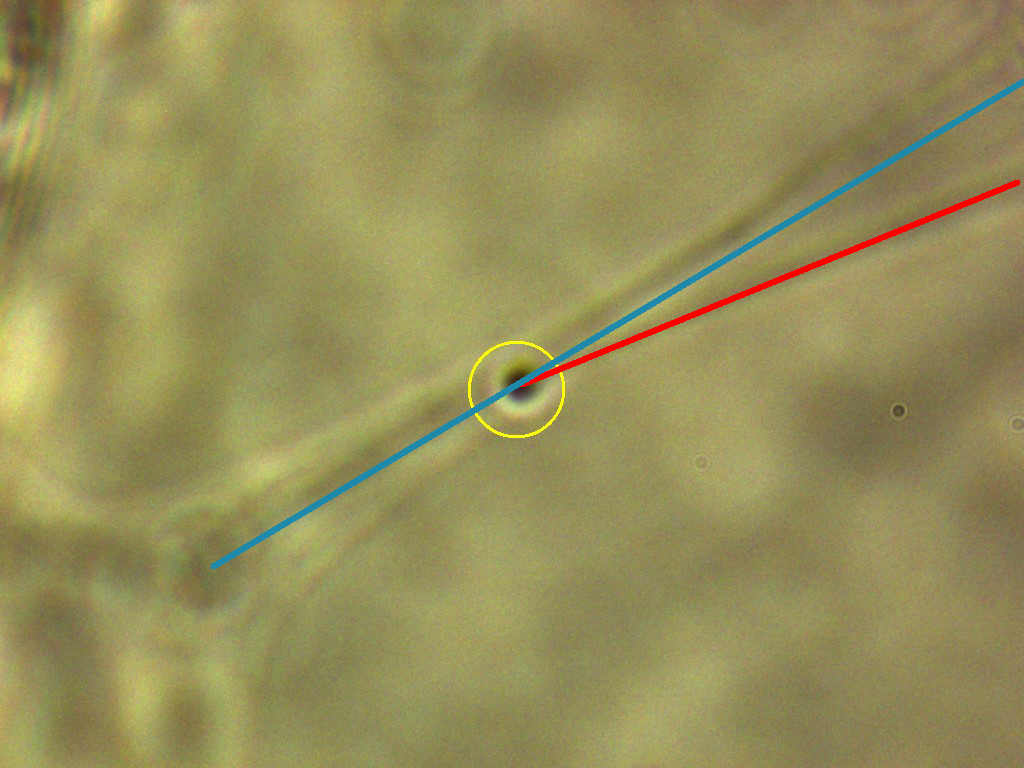
\includegraphics[width = 0.4\textwidth]{pictures/vesikel_overlap.png}
        \caption{Das über der blauen Straße platzierte Vesikel springt bei Deaktivierung der optische Falle auf seine Ausgangsposition auf der Straße am rechten Ende der roten Linie zurück.}
        \label{fig:vesikel_overlap}
        \end{figure}
        %
        \FloatBarrier 
        %
        \newpage
        Auch beim Entfernen der Vesikel von der Straße sind diese jedoch noch beweglich, da die Myosin-Motoren weiterhin funktionieren. In der Nähe einer Kreuzung ist so das schnelle verschieben der 
        Myosin-Motoren entlang der Kreuzung durch Verschieben des Vesikels, wie in Abbildung \ref{fig:vesikel_sprung} schematisch eingezeichnet, möglich.
        %
        \FloatBarrier
        %
        \begin{figure}[h]
        \centering
        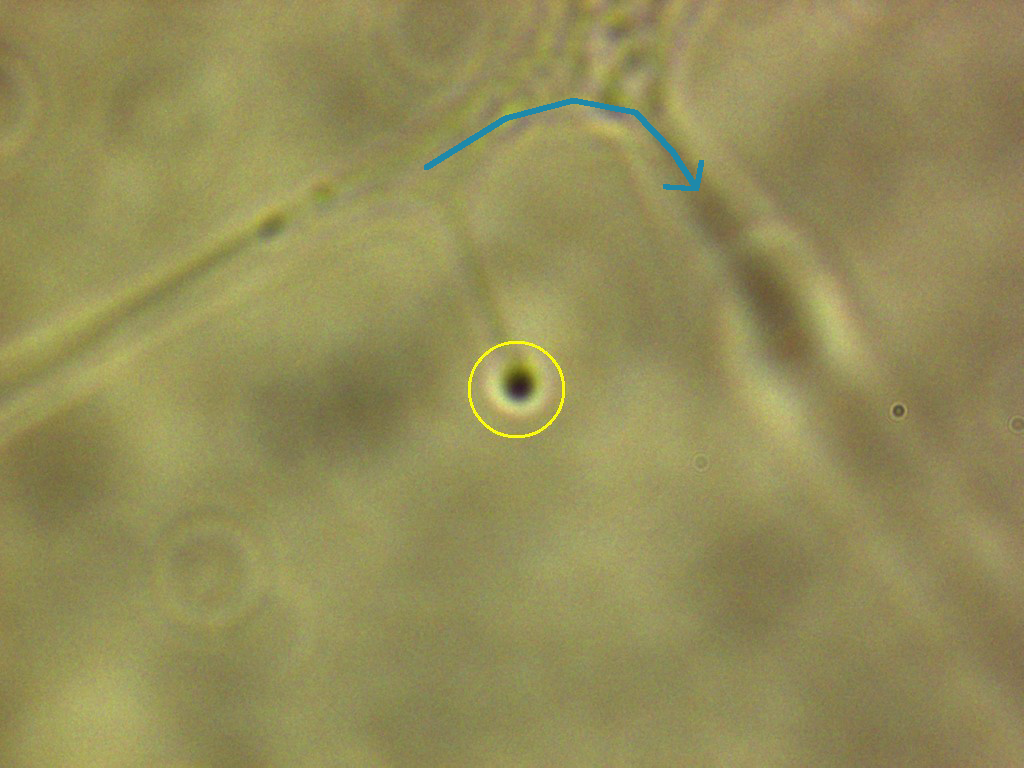
\includegraphics[width = 0.4\textwidth]{pictures/vesikel_transport.png}
        \caption{Bei der gegebenen Vesikelposition können die Myosin-Motoren entlang der Kreuzung auf die andere Straße verfahren.}
        \label{fig:vesikel_sprung}
        \end{figure}
        %
        \FloatBarrier 
        %
        Durch Platzierung der optischen Pinzette über einer Actin-Straße und sukzessivem Erhöhen der Laserleistung ist ein Stopp des Vesikeltransports bei einer Laserleistung von \SI{63}{\milli\watt} zu 
        beobachten. Dies entspricht einer aufgrund der schlechten Kalibrierungsmessungen nur abzuschätzenden Fallensteifigkeit von einigen wenigen \SI{10e-6}{\newton\per\metre}. 